\documentclass[prl]{revtex4}
%\documentclass[prl,twocolumn]{revtex4}

\usepackage{ORI_Group_style}
\usepackage{siunitx}


\graphicspath{{./figs/}}


\begin{document}

\title{Photophysics of Nitrogen Vacancy centres in Nanodiamonds}
  
\author{Reece P. Roberts$^{1,2}$}
\author{Author2$^{1,2}$}

\affiliation{$^1$ Department of Physics \& Astronomy, Macquarie University, NSW 2109, Australia}
\affiliation{$^2$ ARC Centre for Engineered Quantum Systems, Macquarie University, NSW 2109, Australia}


\begin{abstract}
NVs are cool because they do cool sciency stuff.
All cool stuff comes from NV-.
People use 532 excitation to increase charge polarisation so they can optimise cool stuff and neglect NV0.
They looked at it with only one excitation wavelength at a time. 
Clearly charge polarisation depends on wavelength.
So clearly quenching must occur with second wavelength.
Must understand all of this stuff to intergrate NVs into other systems that use lasers.
\end{abstract}

\maketitle

\section{Introduction}

The Nitrogen Vacancy (NV) centre is is a point defect consisting of a nitrogen-vacancy lattice pair embedded along the [111] axis of a diamond (???ref1). The NV centre has two stable charge states, the neutral charge state (NV$^0$) and the negatively charged state (NV$^-$), with photo-induced interconversion between these two states (???ref2). The NV$^-$ charge state is an intensively studied material that has shown a wide range of applications in both Physics and Biology due to it's high stability and interesting optical properties. Biologists have used them extensively for biolabelling and imaging of internal biological structures (???ref3 and 4). Meanwhile, physisits have been investigating their use in a wide range of nanoscale sensing and quantum sensing applications(???ref5). By exploiting the quantum mechanical interactions of the defects internal spin state, room temperature quantum effects can be observed in the NV$^-$ centre providing a platform to study a wide variety of quantum manipulation protocols (???ref6). However, these desirable effects rely solely on the properties arising from the NV$^-$ charge state and in most applications the excitation wavelength is chosen to be around 510-540nm, as this region was shown to have the highest charge state polarisation (ref7???). By using a single optimised excitation wavelength the impact of the neutral charge state NV$^0$ could be neglected despite the optimal charge state polarisation limited at $75\%$. \textbf{Summary: Introduce NV, Show that NV- is the important charge state, lead that we neglect NV0 by exciting with 532nm}

In cases where only the single excitation laser is used the NV centre has been long stated to be extremely robust, with no bleaching or blinking under normal conditions(ref8???). However, in many cases once a second probe laser is used in an experiment the fluorescence of the NV centre is dramatically quenched(ref9???), preventing further applications and systems that require additional laser wavelengths. The quenching of fluorescence has been observed and described by numerous potential mechanisms, including (list here???1). In contrast to many of these mechanisms we are probing in a non resonant continuous-wave regime of a few 10s of milliwatts eliminating many of the above mechanisms that rely transient mechanisms or high intensities fields. In addition, we are collecting the fluorescence of both charge states and do not believe that the NV$^0$ charge state can be neglected in a steady state regime. \textbf{Summary: NV is good when used alone, a second laser field leads to quenching of fluorescence, has been explained by many mechanisms but mostly look at only NV$^-$, NV$^0$ must be playing a role.}

In this paper we investigate the quenching effects of the NV centre fluorescence under near infra-red (NIR) exposure in order to provide insight into the charge and spin state photo-dynamics. From our analysis we found that the quenching mechanism is driven by the continuous charge state transfer between NV$^0$ and NV$^-$ providing increased channels for non radiative decay from the excited states. By understanding the underlying processes we aim to apply particular initialisation processes to increase the spin and charge state polarisation of the NV centre. This will lead to direct enhancements of applications such as STED like imaging and for enhancing state preparation for NV based quantum technologies.
\textbf{Summary: Summary of what we aim to do}
\todo{Should I add examples of further applications and systems that require additional laser wavelengths}

In our experiment, 100nm nanodiamonds are dispersed on a glass coverslip placed on the sample plane of a custom built scanning confocal microscope. The NV centres are pumped with a 532nm continuous wave laser after focusing through a x.xNA, Brand, type immersion objective lens ???3. The 780nm laser is combined and then superimposed with the 532nm laser before the objective lens. The fluorescence is collected through the same objective and sent to either a fibre spectrometer or a fibre coupled APD that collects all wavelengths between $550-\SI{700}{nm}$. A permanent neodymium magnet was placed on a moveable arm above the sample plane so that a large non zero magnetic field could be brought in close proximity to the nanodiamond in order to investigate the effect of mixing the spin state of the NV$^-$ ground states. The setup is shown in Fig. \ref{FigSetup}.

\begin{figure}[t]
  \centering
  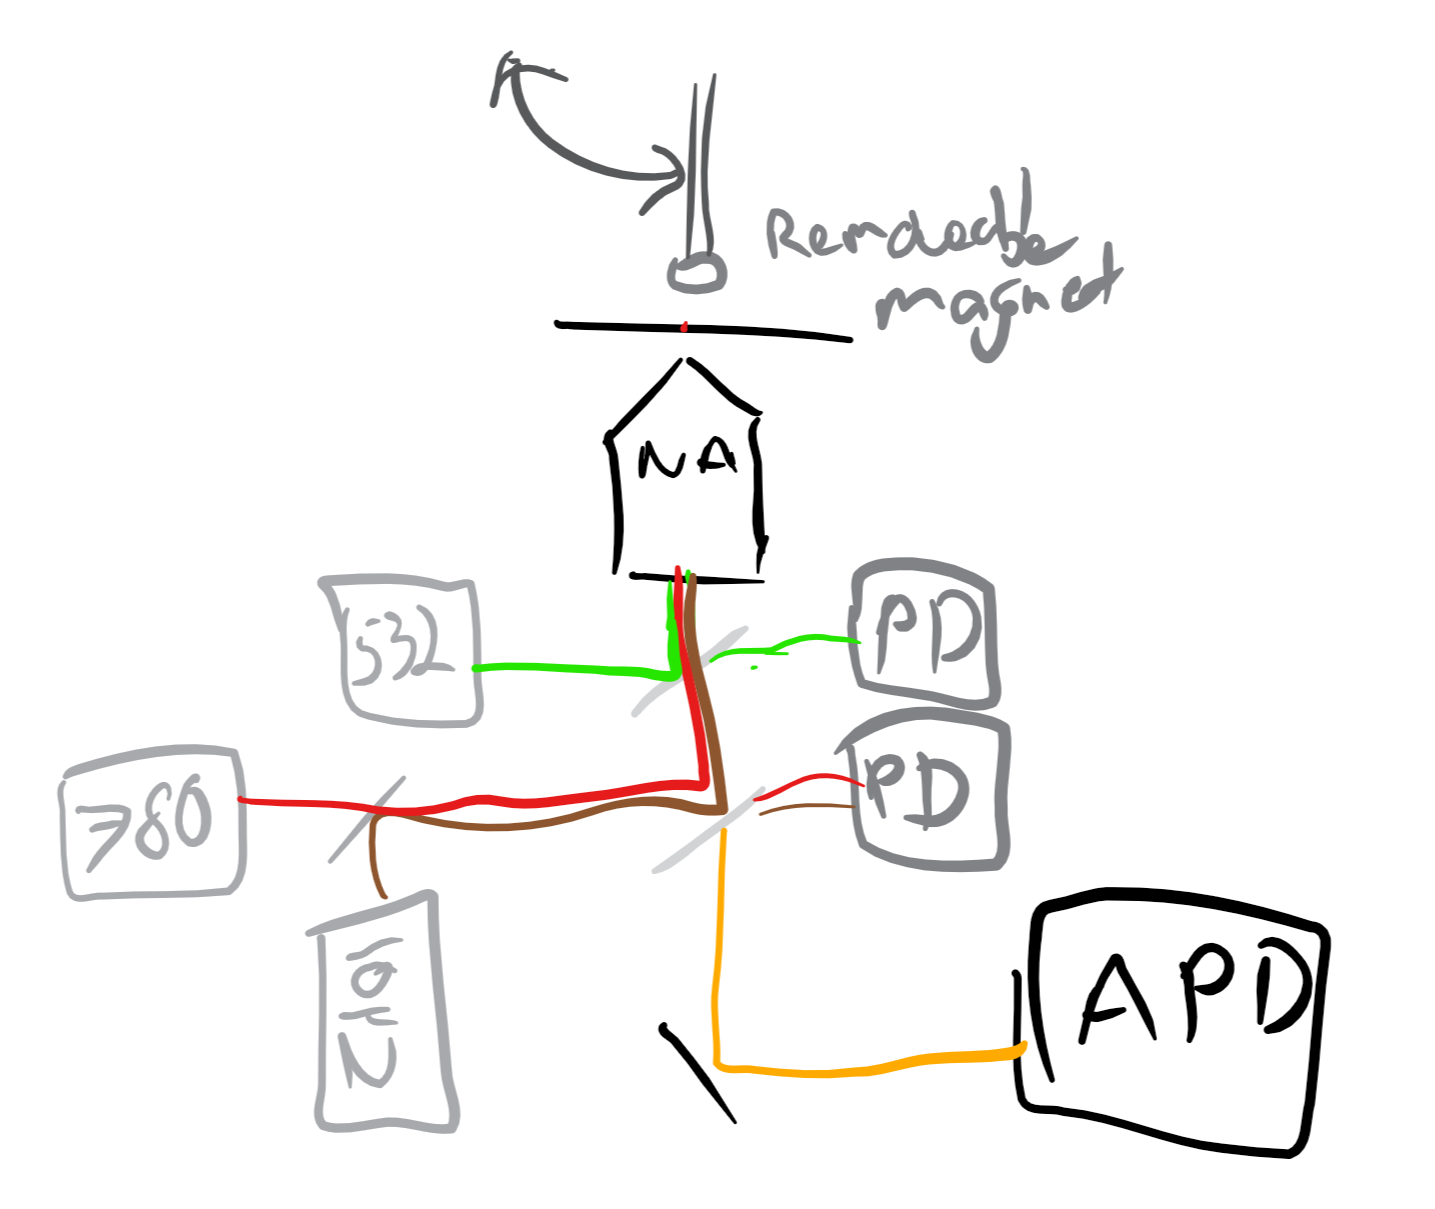
\includegraphics[width=0.3\textwidth]{Setup.png} 
 \caption{\textbf{Experimental approach.} This is the setup ???} \label{FigSetup}
\end{figure}

We first examined the spectral response of excited NV centres under NIR illumination. The NV was excited with ???mW of 532nm and the NIR power dependence of the florescence spectrum was acquired and can be observed in Figure ???.

\begin{figure}[H]
  \centering
  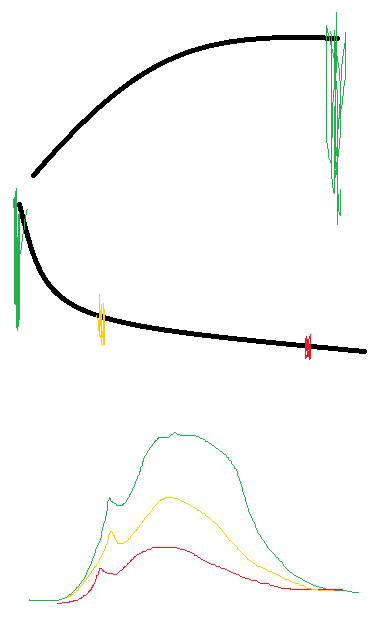
\includegraphics[width=0.4\textwidth]{Spectra.png} 
 \caption{\textbf{Experimental data.} \textbf{a.} This is the data swap a and b???} \label{FigSpectra}
\end{figure}

Both the fluorescence of NV$^0$ and NV$^-$ can be observed to be decreasing with increased NIR power. Additionally, there does not appear to be a significant charge transfer between the two charge states. Exact charge polarisation cannot be identified from the spectra due to the inability to spectrally separate the two charge states. It is clear however from the spectra that the quenching of fluorescence cannot be explained by simply investigating the negative charge state and neglecting the neutral charge state.

In order to investigate the entire photo-dynamics of the NV centres we used the APD to observe the fluorescence over a much larger parameter space. For each nanodiamond the saturation curve of the NV centre is measured. The power dependence of the fluorescence for the $\SI{785}{nm}$ illumination wavelength is then measured for five powers of the $\SI{532}{nm}$ excitation laser. The neodymium magnet is placed $\approx \SI{0.5}{mm}$ above the sample plane of the confocal microscope in order to mix the spin state of the NV- charge state. The above set of measurements are then repeated to provide more information on the internal spin state of the system. For each nanodiamond we obtain a series of plots that can be observed in figure \ref{FigData}.

\begin{figure}[H]
  \centering
  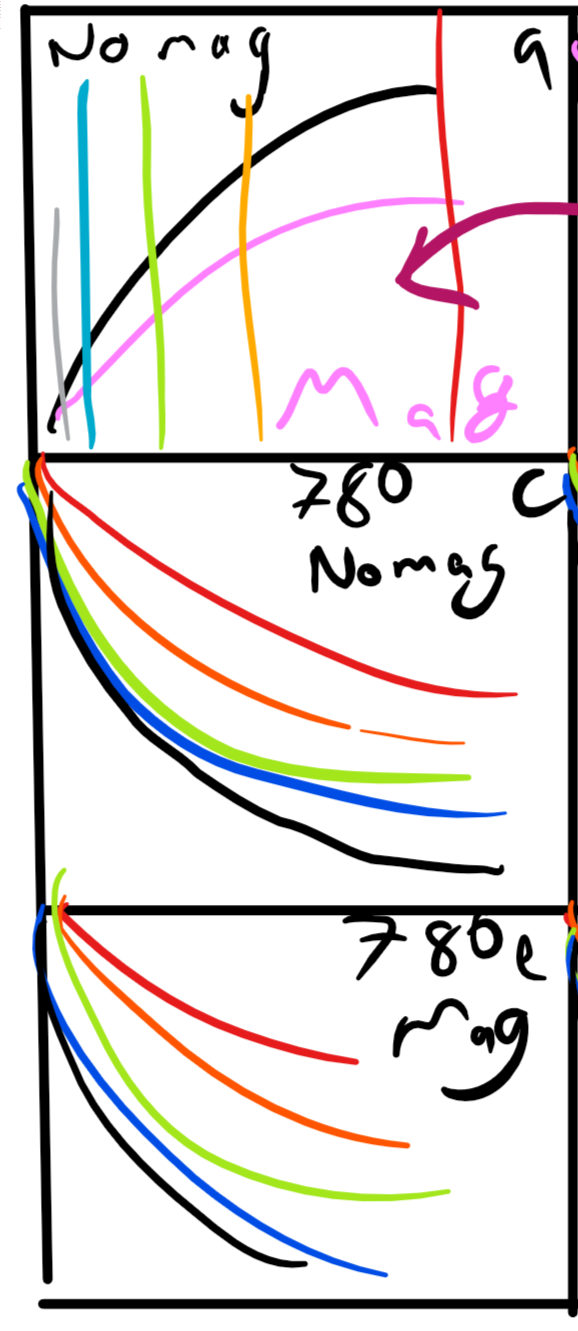
\includegraphics[width=0.4\textwidth]{Data2.png} 
 \caption{\textbf{Experimental data.} \textbf{a.} This is the data swap a and b???} \label{FigData}
\end{figure}

To determine the intrinsic photophysics of our nanodiamonds we developed an 8 level rate equation model using established physics of the NV centre that incorporates both the ionisation and recombination mechanisms as well as the STED like mechanisms. It is important to note that whether the STED like effect is simply non radiative decay from the excited to ground triplet state ref34??? or is mediated through a new fast decaying dark band ref35??? the mechanisms reduce to identical rate equations. The free parameters of the model were varied in order to determine the most likely photo-dynamics of the system. ??? submodels were investigated and the most likely model was identified by the Akaike information criteria. In the body of this paper only the most likely model selected by the Aikike information criteria is discussed, however, the full analyses of all the potential photo-dynamic models, are discussed in the Appendix. The model identified by the Aikike information criteria indicates that the quenching process occurs through continuous charge state transfer between NV$^0$ and NV$^-$ leading to increased channels for non radiative decay from the excited states of the NV centre. Additionally whilst the model is kept quite general and unconstrained the final fitting parameters of the model are consistent between many NV centres and provide values that are physical and are consistent with measurments observed in the literature. It is important to note that whilst a STED like mechanism can fit the quenching data in some situations, once the internal spin of the system is investigated the analysis for this mechanism is no longer accurate. The energy level structure and fitting parameters for the processes leading to the quenching observed through the ionisation and recombination process is shown in Figure \ref{FigEnergyLevelsNV}.

\begin{figure}[H]
  \centering
  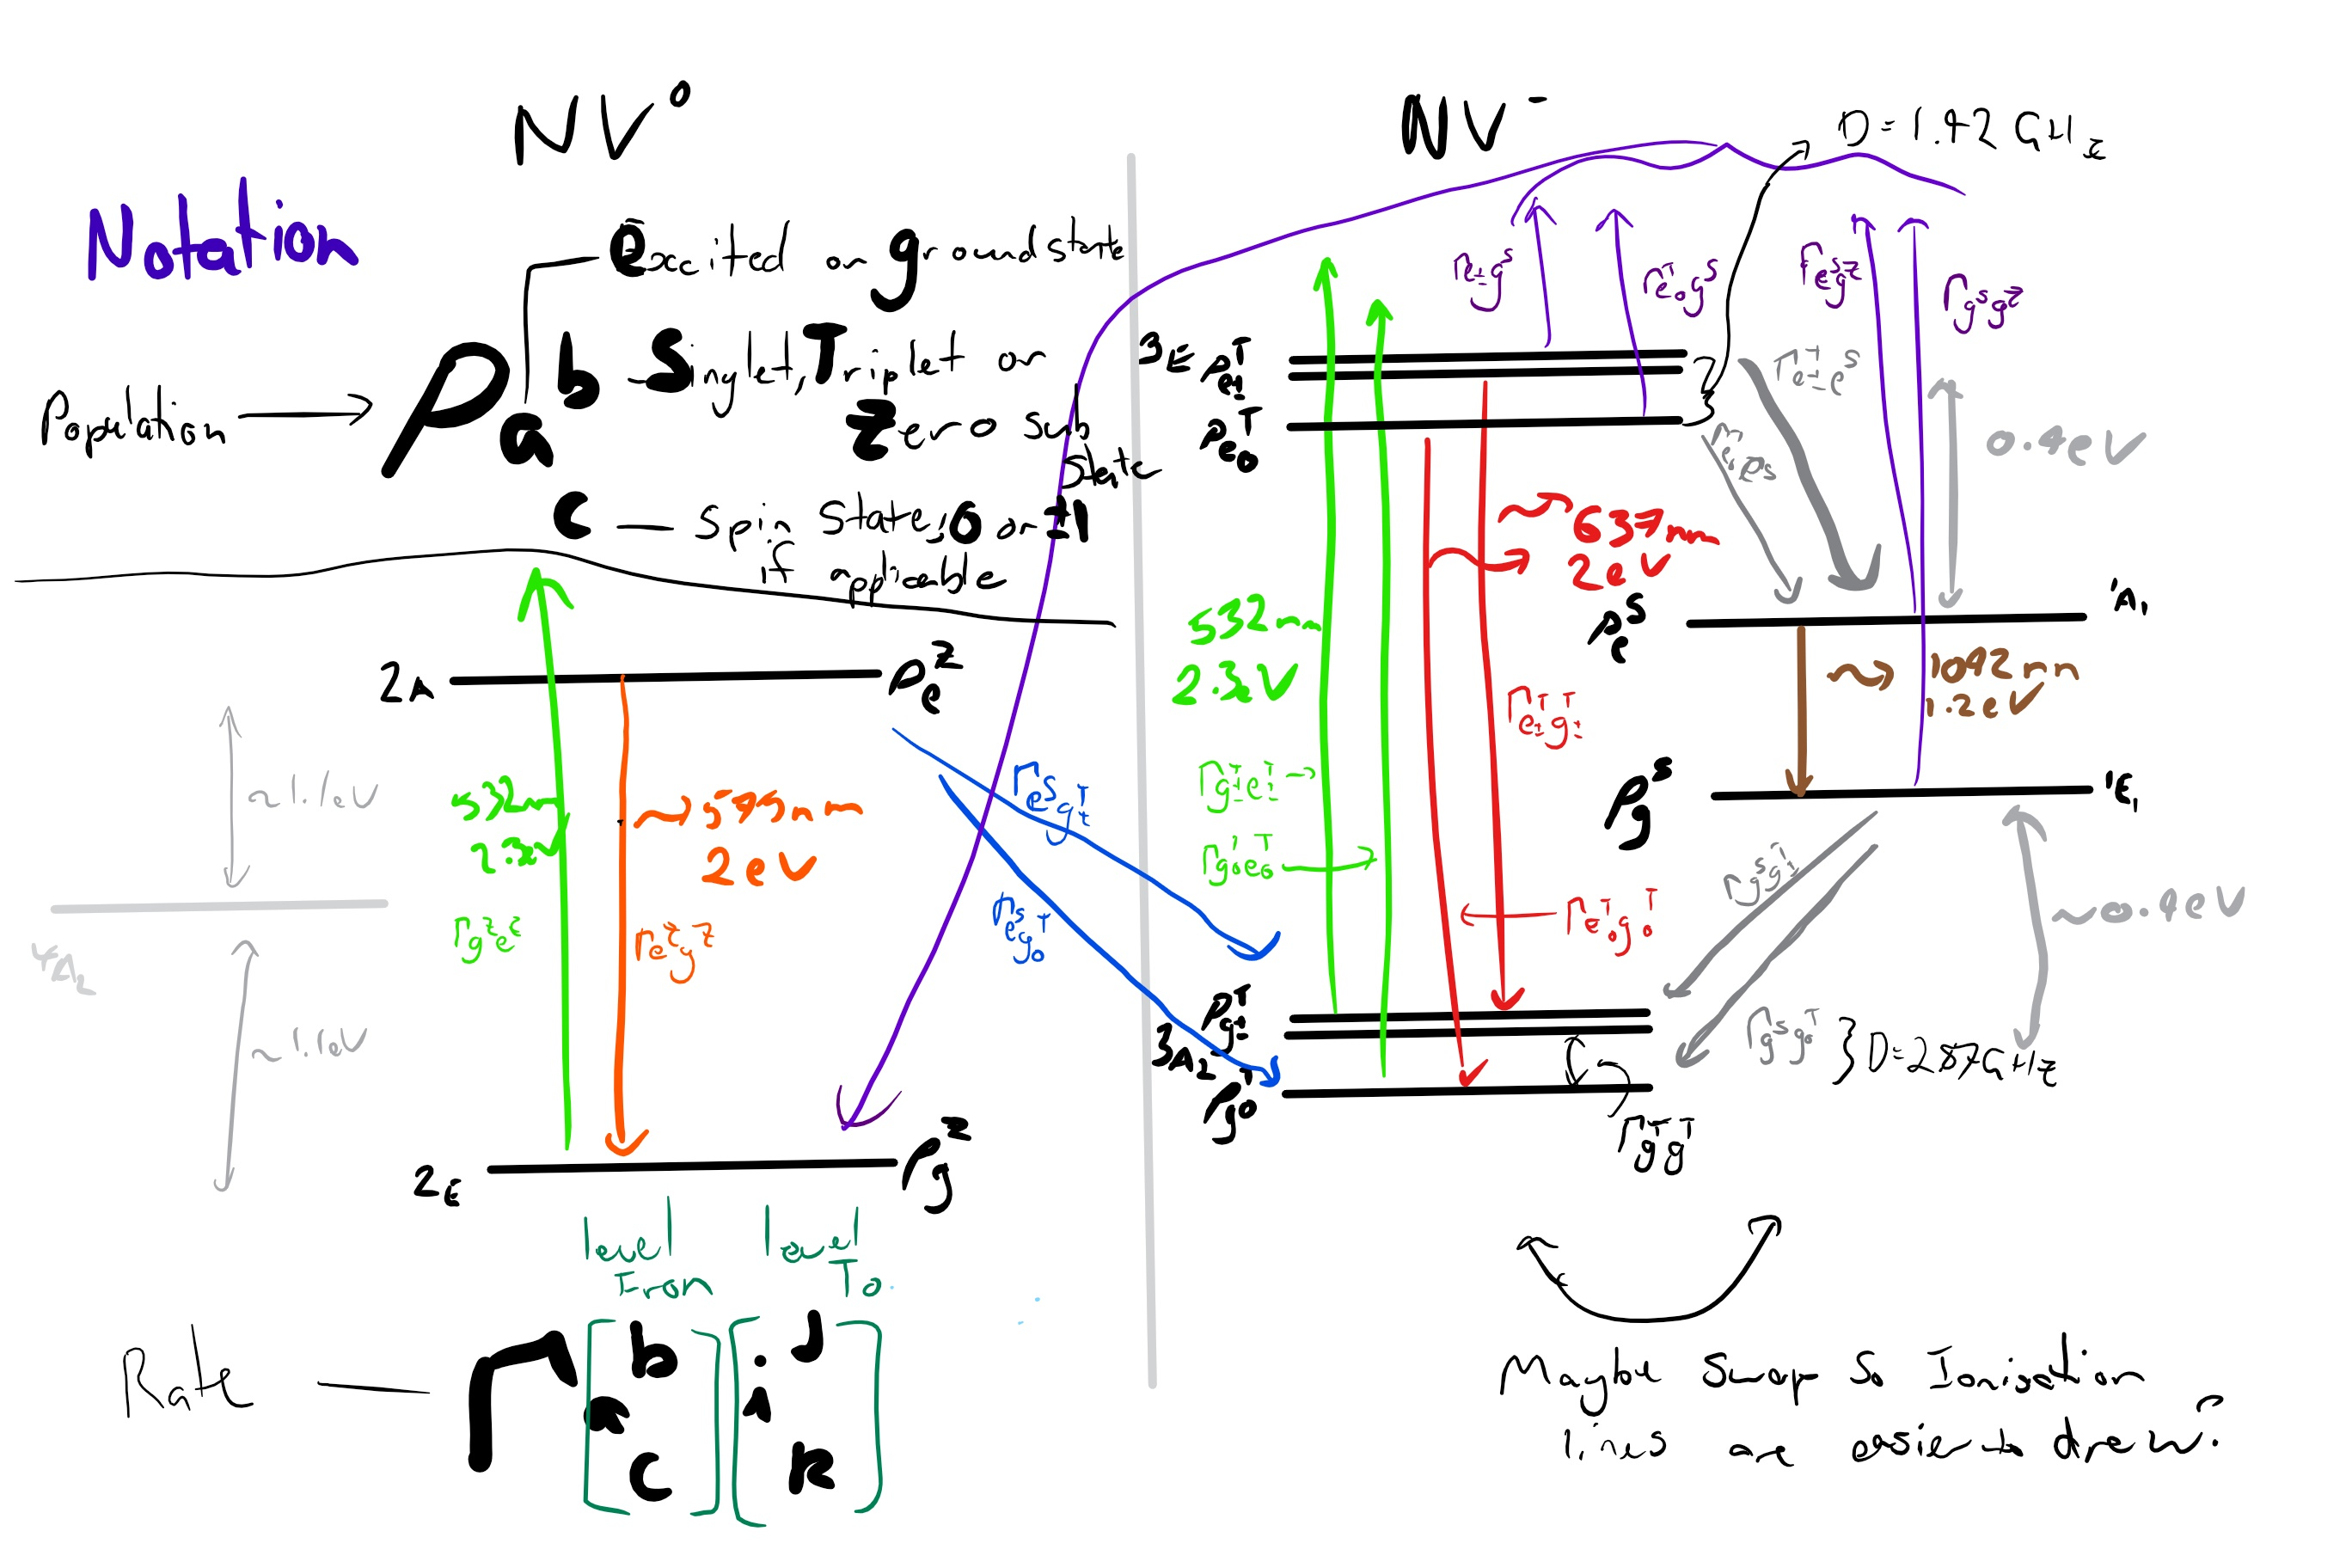
\includegraphics[width=0.4\textwidth]{NVjpg.jpg} 
 \caption{Energy levels of the NV centre.} \label{FigEnergyLevelsNV}
\end{figure}

The populations of the energy levels can be solved under steady state conditions and the fluorescence intensity is given by the population of each excited state and their fluorescence decay rates,

\begin{equation}
\SI{}{F} = \left(\rho_{e^{T}_\pm}\times\Gamma_{e^T_{\pm}g^T_{\pm}} +\rho_{e^{T}_0}\times\Gamma_{e^T_{\pm}g^T_{\pm}}\right)+\left(\rho_{e^Z}\times\Gamma_{e^Zg^Z}\right)\times\sigma,
\label{EqnFluoro}
\end{equation}

where F is the fluorescence intensity and $\sigma$ is the ratio between the efficiency of collecting a NV$^-$ photon compared to an NV$^0$ photon, which depends on the fluorescence spectra and the collection window as well as the spectral response of the detector. This was calculated to be $\sigma=1.5$ for our ??? APD with a fluorescence window between $\SI{550}{nm}$ and $\SI{700}{nm}$. For the saturation curves this value can be compared directly against the data with a single scaling parameter, which is related to the effective number of NV centres and collection efficiency, whereas for the NIR quenching data the data can be compared directly by normalising to the fluorescence intensity with no NIR laser power,
\begin{equation}
\SI{}{Fluorescence\ Counts\ (norm}.) = \frac{F(I_{NIR})}{F(0)}.
\label{EqnFluoroCounts}
\end{equation}


The NV$^-$ charge state consists of a ground triplet state $^3A_2$ and an excited triplet state $^3E$, as well as two metastable singlet states $^1E_1$ and $^1A_1$ ref11???. Within the spin triplet states the $m_s = 0$ ans $m_s = \pm1$ spin states are split in energy at zero magnetic field by $D=\SI{2.87}{GHz}$ for the ground triplet and $D=\SI{1.42}{GHz}$ for the excited triplet (Ref12???). The spin transition rate between the ground $m_s = 0$ and $m_s = \pm1$ spin states is given by the spin-lattice relaxation time $T_1$ and has been measured to be $\approx\SI{6}{ms}$ at room temperature and zero magnetic field (ref13???). This spin mixing rate can be dramatically increased by applying a large magnetic field in the vicinity of the NV centre ref14???. In our model the spin mixing rate between the two ground states of the NV$^-$ charge state when there is a magnet present above the nanodiamond is $6\pm \SI{3}{MHz}$.

\todo{I am being vague about the spin mixing rate because because I believe the current explanation of Zeeman splitting the spin sublevels has holes in it. Ask me for more info or look at comment in tex file}
% This explanation would not explain the saturation effect that are observed as you bring in the magnet. Following the Zeeman splitting logic you would expect only one spot where there is large mixing and then you would reduce the mixing as you cross this precise field strength. However this saturation effect may be a result of having a collection of NV centres, however Xavi and Matt observed the same effect with single NV centres. This leads to the belief that the spin mixing may not be due to zeeman splitting and the absolute magnitude of the magnetic field but instead due to the thermal perturbations of the magnet destroying the spin coherence. In any case someone familiar with NV centres will accept this statement anyway. Although the question of why there is no spin mixing on the excited state is still a valid question that I still have no answer for other than it is completely absent from the literature and at this stage (22/12/16) my model does indicated that it does not occur. 	I also had the thought that the spin mixing rate is still increasing as we are bringing in the magnet but the rate is already high enough to spin depolarise the system. This can be checked using the model.
%If they were only capturing NV- or mostly NV- (I Never got a good answer to this question from MAtt and Xavi) then due to a combination of the magnet mixing the spin state, which will give an \~\%30 quenching by it self, and then due to spin dependant ionisation this mixed spin state will lead to a higher Ionisation rate and hence a reduction in NV$^-$ charge state polarisation and reduction in Fuorescence.
 
The principle zero-phonon line between the $^3A_2$ and $^3E$ is centred at 637nm and can be efficiently excited with spin conservation at most wavelengths below 640nm (ref15???). The radiative lifetime of the excited state is $\SI{13}{ns}$ for NV centres in bulk diamond (ref16???) and approximately $\SI{25}{ns}$ for NV centres in nanodiamonds (ref17???). Only a few percent of the Fluorescence is emitted at the ZPL, most fluorescence appears in the phonon side bands between 600 and 800nm.

The excited triplet states can also decay to the excited singlet state, the rate from the $m_s=\pm1$ excited triplet state is $2\pi\times9.4\times10^6\SI{}{GHz} = \SI{16.9}{ns}$, whereas the rate from the $m_s=0$ excited triplet state is almost an order of magnitude smaller at $ 2\pi\times1.8\times10^6 \SI{}{GHz} = \SI{88.4}{ns}$ (ref18???). Whilst it not completely understood why there is a large discrepancy between these decay channels it is noteworthy that this discrepancy is what leads to many of the interesting optical properties of the NV centre. It causes a difference in fluorescence intensity between the two excited spin states which in turn leads to a mechanism for an all optical readout of the centres internal spin state. The excited singlet state has a lifetime of $\approx\si{1}{ns}$ (ref19???) and populates the longer lived ground singlet state and it has been shown to emit fluorescence at a ZPL of $\SI{1042}{nm}$ ref20???. The longer lived ground metastable state has a lifetime of $\SI{150}{ns}$ and decays into the ground the triplet spin state ref21???. It was commonly believed that this population decayed only into the $m_s=0$ spin state, however a recently this is being challenged and it has been claimed that the decay into the ground triplet has a spin state is nanodiamond dependant and only 0.5-0.7\% of the electrons decay into the $m_s=0$ ground state ref22???. Our model is consistent with the observation that the singlet state does not decay only into the $m_s=0$ ground state and only $0.7 \pm 0.2\%$ of the electrons decay into the $m_s=0$ ground state.

As opposed to the rigorous study the NV$^-$ charge state has received the $NV^0$ charge state has often been neglected. However we believe in order to study the NV centre as a whole it must be included. We use the established three level model to describe its intrinsic dynamics. The NV$^0$ charge state consists of of a ground doublet $^2E$ and an excited doublet $^2A$ with a ZPL at $\SI{575}{nm} = \SI{2.156}{eV}$.  It can be efficiently excited at most wavelengths below $\SI{675}{nm}$ ref23??? and has a radiative lifetime of $\Gamma_{e^Zg^Z} = 19\times2 \SI{}{ns}$ ref26???. The exact excitation cross section is unknown, however, the ratio of excitation cross sections between NV$^0$ and NV$^-$ can be measured by looking at their relative emission intensities. In addition, since the quantum efficiency of NV$^0$ and NV$^-$ is $\approx 1$ then the ratio of excitation cross sections is given by the ratio of emission cross sections giving $\Gamma_{g^Ze^Z} = \frac{1}{3} \Gamma_{g^Te^T}$ ref25???. Differing from NV$^-$, NV$^0$ does not have detectable magnetic resonances associated with its degenerate spin doublet ground and excited states ref24???. Only a few percent of the fluorescence is emitted in the ZPL, whereas most fluorescence appears in the phonon side bands between 550 and 750nm. However, no ODMR or optical readout of this metastable quartet have been measured and it is expected to have negligible impact on the photo-physics of the NV centre and as such has been neglected from our analysis. 

\todo{I think I doubled this value because NV- lifetimes were doubled in ND as compared to bulk and the lifetime I found was in Bulk diamond. Either need to find value for ND's or argue that it should also increase the same way as NV- did...}

\subsection{Ionisation \& Recombination}
To convert between the two charge states we need to examine both the Ionisation process from NV$^-$ to NV$^0$ and the recombination process from NV$^0$ to NV$^-$. The desirable effects of the NV centre rely solely on the properties arising from the NV$^-$ charge state and as a result a standard $\approx \SI{532}{nm}$ excitation laser used in NV centre applications is chosen so that it produces the highest charge state polarisation in an effort to optimise the effect and allow any effects due to the $NV^0$ charge state to be neglected (ref7???). However, an additional laser is going to alter this maximised charge state polarisation. 

\subsection{Ionisation Process}
Ionisation from NV- to NV0 occurs in a two step process as shown in Fig. \ref{FigChargeConversiona}.

\begin{figure}[H]
  \centering
  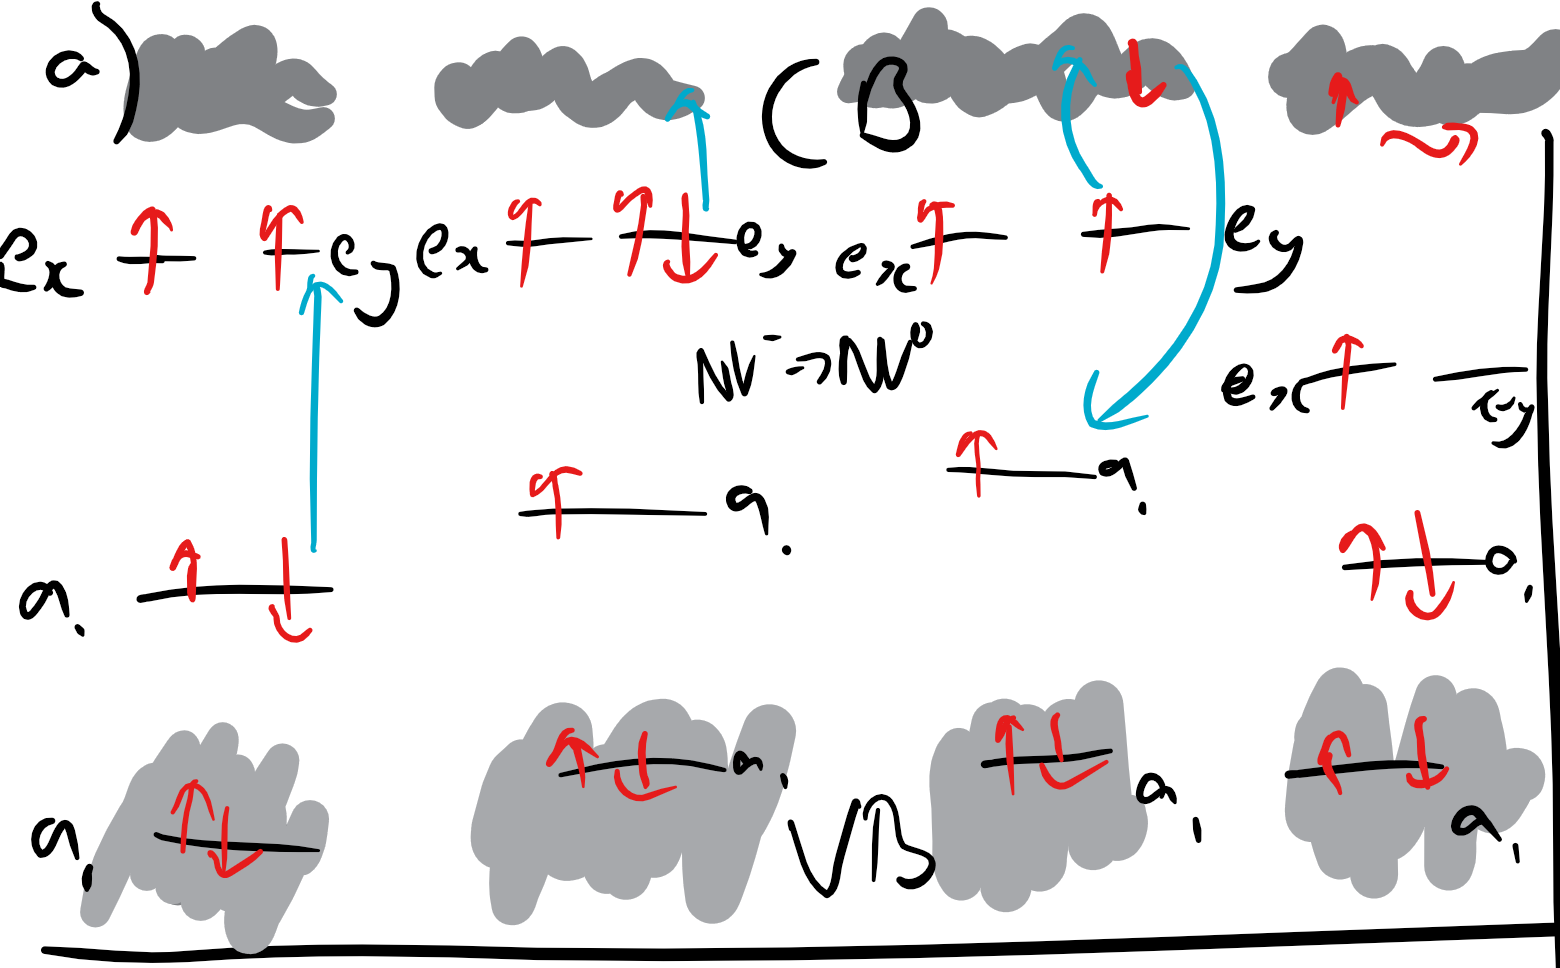
\includegraphics[width=0.4\textwidth]{ChargeConversiona.png} 
 \caption{\textbf{Ionsation Processes.} \textbf{a,} Ionisation from NV$^-$ to NV$^0$ electron view \textbf{b,} Ionisation pathways traditional view.} \label{FigChargeConversiona}
\end{figure}

First a photon must excite an electron into the excited $^3E$ state of the NV$^-$. The electron can then be excited again into the conduction band leading to an Auger ionisation process which strips an electron from the centre converting it into the NV$^0$ charge state in its ground state configuration (ref28???). This two step process has only been investigated with a single excitation laser which leads to an ionisation rate that is quadratic with excitation power and can no longer occur at wavelength greater than the ZPL of the transition. However, we believe this process can be mediated by two lasers, one that strongly excites the transition and one that strongly ionises the electron leading to the Auger ionisation process. One would initially assume that the ionisation mechanism would be spin independant, however these energy levels already show a spin dependant nature towards the singlet states that leads to the spin polarisation properties of the NV$^-$. As a result we investigated the possibility that the interactional cross sections of the excited NV$^-$ centre can be spin dependant. Indeed, the most likely model selected by the Akaike criteria indicates that the ionisation process occurs $5.1\pm0.2\times$ faster from the $m_s=0$ excited charge state than from the $m_s=\pm1$ for both 532nm and 785nm lasers. The corresponding ionisation rates out of the $m_s = 0$ excited spin states are $11.4\pm\SI{0.8}{MHz/mW}$ and $7.866\pm\SI{0.005}{MHz/mW}$ at 532nm and 785nm respectively. 


\subsection{Recombination Process}
The recombination process from NV$^0$ to NV$^-$ also occurs in a two step process and is shown in Fig. \ref{FigChargeConversionb}.

\begin{figure}[H]
  \centering
  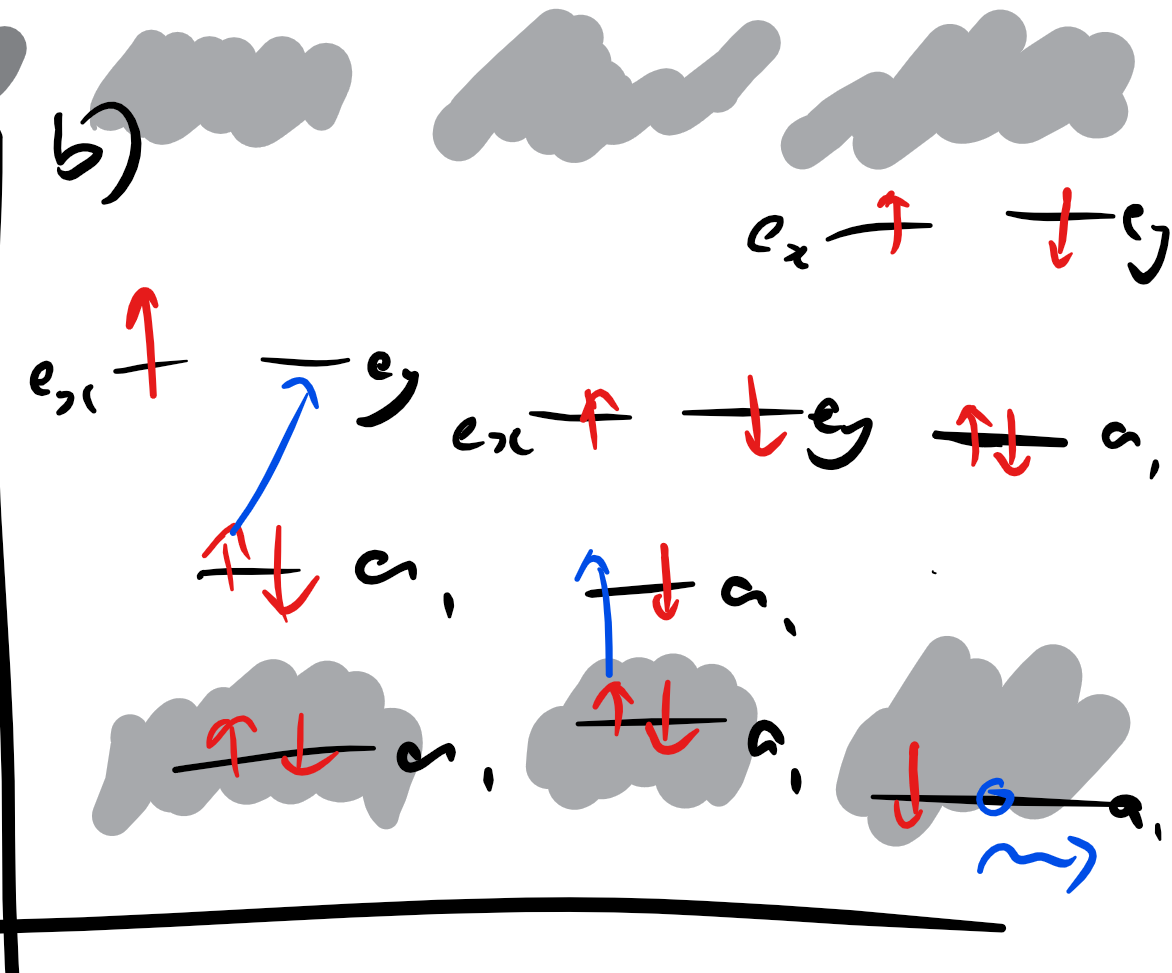
\includegraphics[width=0.4\textwidth]{ChargeConversionb.png} 
 \caption{\textbf{Recombination Processes.} \textbf{a,} Recombination from NV$^-$ to NV$^0$ electron view \textbf{b,} Recombination pathways traditional view.} \label{FigChargeConversionb}
\end{figure}

First a photon must excite an electron in the NV$^0$ charge state into the excited $^2A$ state. A second photon can then be excited from the valence band into the $^2E$ ground state which provides the extra electron to the centre converting it into the NV$^-$ charge state in its ground state configuration (ref29???). Currently there is no evidence to indicate which spin state the NV$^-$ charge state will now be populated in, however it has recently been observed that the ionisation, recombination process is a spin depolarising process indicating a non negligible component in the $m_s=\pm1$ spin state ref30???. In our analysis we observe that the rate of recombination from NV$^0$ to NV$^-$ is $180\pm\SI{90}{MHz/mW}$ at 532nm and $18\pm\SI{2}{MHz/mW}$ at 785nm. Additionally the model indicates that this process is spin depolarising such that the ratio into the $m_s=0$ ground state of the NV$^0$ is $49.0\pm0.06\%$ for both laser wavelengths.

\section*{Acknowledgements}

....
%%%%%%%%%%%%%%%%%%%%%%%%%%%%%%%%%%%%%%%%%
%%%%%%%%%%%%%%%%%%%%%%%%%%%%%%%%%%%%%%%%%
%%%%%                                                                                                   %%%%%
%%%%%                                       APPENDIX                                          %%%%%
%%%%%                                                                                                   %%%%%
%%%%%%%%%%%%%%%%%%%%%%%%%%%%%%%%%%%%%%%%%
%%%%%%%%%%%%%%%%%%%%%%%%%%%%%%%%%%%%%%%%%

%
\appendix

\section{model}
\begin{eqnarray}
\dot{\rho_{e^{T}_0}} & = &-\rho{e^{T}_0}\left(\Gamma_{e_0^Tg_0^T}+\Gamma_{e_0^Te^S}+Ion_0^{780}\times I_{780}+Ion_0^{532}\times I_{532}+STED^0_{780}\times I_{780}+STED_0^{532}\times I_{532} \right) \\
&& +\rho_{g^{T}_0} \left( A\times I_{532}\right)\\ 
\dot{\rho_{e^{T}_\pm}} & = &-\rho_{e^{T}_\pm}\left(\Gamma_{e_{\pm}^Tg_{\pm}^T}+\Gamma_{e_{\pm}^Te^S}+Ion^{\pm}_{780}\times I_{780}+Ion_{\pm}^{532}\times I_{532}+STED_{\pm}^{780}\times I_{780}+STED_{\pm}^{532}\times I_{532}\right)\\
&& \rho_{g^{T}_\pm}\left(A\times I_{532}\right)\\
\dot{\rho_{g^{T}_0}} & = & \rho_{e^{T}_0} \left(\Gamma_{e_0^Tg_0^T}\right)+\rho_{g^Z} \left(\kappa\Gamma_{g^S}\right)+\Gamma_{SF}\left(\rho_{g^{T}_{\pm}}-\rho_{g^{T}_0}\right)-\rho_{g^{T}_0} \left( A\times I_{532}\right)+\rho_{e^Z}\left(\mu R_{532}+\nu R_{780}\right)\\
& &+\rho{e^{T}_0}\left(STED^0_{780}\times I_{780}+STED_0^{532}\times I_{532} \right)\\
\dot{\rho_{g^{T}_\pm}} & = & \rho_{e^{T}_{\pm}} \left(\Gamma_{e_{\pm}^Tg_{\pm}^T}\right)+\rho_{g^Z} \left(\left(1-\kappa\right)\Gamma_{g^S}\right)+\Gamma_{SF}\left(\rho_{g^{T}_0}-\rho_{g^{T}_{\pm}}\right)-\rho_{g^{T}_{\pm}} \left( A\times I_{532}\right)+\rho_{e^Z}\left(\left(1-\mu\right) R_{532}+\left(1-\nu\right) R_{780}\right)\\
& &+\rho{e^{T}_{\pm}}\left(STED^{\pm}_{780}\times I_{780}+STED_{\pm}^{532}\times I_{532} \right)\\
\dot{\rho_{e^S}} & = & \rho{e^{T}_0}\left(\Gamma_{e_0^Te^S}\right)+\rho{e^{T}_{\pm}}\left(\Gamma_{e_{\pm}^Te^S}\right) - \rho_{e^S}\left(\Gamma_{e^Sg^S}\right)\\ 
\dot{\rho_{g^S}} & = & \rho_{e^S}\left(\Gamma_{e^Sg^S}\right)-\rho_{g^S}\left(\Gamma_g^S\right) \\ 
\dot{\rho_{e^Z}} & = & \rho_{g^Z}\left(\sigma A\times I_{532}\right)-\rho_{e^Z}\left(\Gamma_{e^Zg^Z}+R_{532}+R_{780}\right)\\ 
\dot{\rho_{g^Z}} & = & -\rho_{g^Z}\left(\sigma A\times I_{532}\right)+\rho{e^{T}_0}\left(Ion_0^{780}\times I_{780}+Ion_0^{532}\times I_{532}\right)+\rho_{e^{T}_\pm}\left(Ion^{\pm}_{780}\times I_{780}+Ion_{\pm}^{532}\times I_{532}\right).
\label{EqnArray}
\end{eqnarray}


\section{Unknown Questions and Assumptions }
In developing the rate equation model there are three unanswered questions that will affect the photo-physics of the system that need to be investigated. For each question a variety of conjectures were developed in order to generate an array of sub-models. The group of sub-models are obtained by generating the complete set of permutations of the given conjectures. The models are then compared with each other using the Akaike Information Criteria, which provides a measure of the comparative likelihood of a model to fit the given data.

The first question is to determine whether the STED like quenching mechanism itself can explain all of the photo-dynamics of the system or if it necessary to include the ionisation, recombination mechanism. Four permutations are investigated to fit the data; Using only a STED like mechanism which will inevitably ignore the NV$^0$ charge state, using a STED like mechanism as well as an ionisation and recombination process mediated only by the $\SI{532}{nm}$ excitation laser, using the STED like mechanism and the ionisation and recombination process mediated by both the $\SI{532}{nm}$ excitation laser and the NIR laser and lastly by leaving out the STED like process and using only the ionisation and recombination process mediated by both the $\SI{532}{nm}$ excitation laser and the NIR laser.
Secondly, it is unclear how the electrons recombine into the into the NV$^-$ ground state from both the metastable state and from the NV$^0$ charge state, the traditional notion and our first conjecture is that the singlet rate decays only into the $m_s=0$ spin state and that the there is no favourable transition for the recombination process, for generality we also provide a case in which there is no limitation on either combination ratio. \todo{Optional:We are however assuming in both of these cases that the presence of a strong magnet field does not effect the energy level favourability of the ground triplet state and hence provide another case where the recombination ratios may change with the presence of the magnet. (I cam up with this effect to explain the \%50 quenching observed by Xavi and Matt due to only the magnet but I beleive that can now be explained without this mechanism. If you want some details about why I think you can actually get \%50 due to the magnet just ask me} Lastly, no investigation has been made into the spin dependency of the ionisation process. These energy levels already exhibit spin dependant rates to the metastable singlet state, and additionally there is a permanent dipole that is an order of magnitude larger for the $m_s = \pm1$ excited spin state than there is for the $m_s=0$ spin state which we believe has the potential to lead to a spin dependant ionisation process ref36???. As a result we do not want to limit our potential models to having only a spin independent ionisation process and hence provide two more cases; a completely spin independent case and a case where spin independent process has the same ratio for both the $\SI{532}{nm}$ and NIR laser. The sub-models were generated from these assumptions and fitted to the data. A summary of all of the various conjectures and sub-models as well as fitted parameters can be found in Tab. or Fig.

\begin{figure}[H]
  \centering
  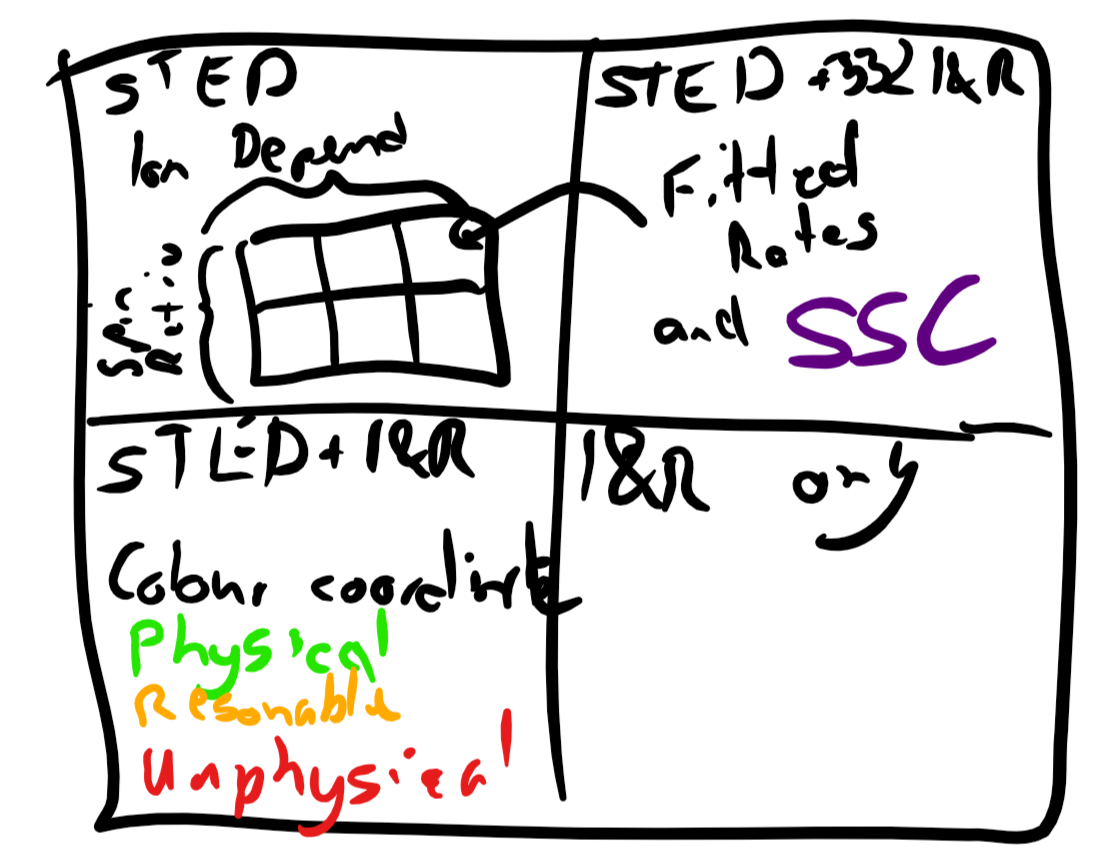
\includegraphics[width=0.4\textwidth]{SubModels.png} 
 \caption{\textbf{Overview of assumptions.} Need to determine a good way of presenting this information.} \label{FigSubModels}
\end{figure}

\section{Quenching Models}
In order to determine the intrinsic photophysics of our nanodiamonds we developed an 8 level rate equation model that incorporates both the ionisation and recombination mechanisms as well as the STED like mechanisms. The free parameters of the model were varied in order to determine the most likely dynamics of the system. Six submodels were investigated and the most likely model was identified by the Akaike information criteria. The six models can be seen in figure \ref{FigModels}.

\begin{figure}[H]
  \centering
  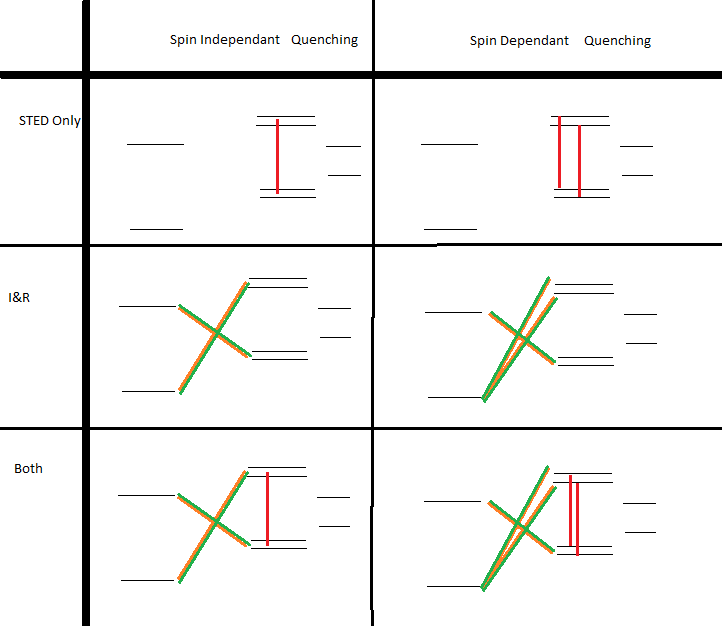
\includegraphics[width=0.5\textwidth]{models.png} 
 \caption{\textbf{Experimental models.} \textbf{a.} This are the six models we looked at} \label{FigModels}
\end{figure}


The models can separated by their underlying quenching mechanism whether it be a STED like process, an Ionisation and Recombination process or a combination of the two. These three groups can then be split in two depending on if the model is a spin dependent quenching model or a spin independent quenching model. Below is a short description of each of the separate model types, for a comprehensive description of the rate equations and models refer to the supplementary material.

\subsubsection{STED like models}
The STED like models are models that describe the quenching of the fluorescence through a true stimulated emission process or even by a  processes that are mediated though an extra metastable fast decay state of the NV$^-$ centre ref???.

\subsubsection{Ionisation and Recombination models}
The ionisation and recombination models relies on the two step processes that convert the charge state of the NV centre. Each time the NV centre is excited the flouresence of the NV centre is reduced due to the increased non radiative decay channels enabled by the conversion of charge state of the NV centre.

\subsubsection{Spin Dependency}
In each of the above mechanisms the quenching of the fluorescence from the NV$^-$ charge state can occur from either the $m_s=0$ or $m_s=\pm1$ excited state. One would initially assume that the ionisation and STED like mechanisms would be spin independant, however these energy levels already show a spin dependant nature towards the singlet states that leads to the spin polarisation properties of the NV$^-$. As a result we investigated the possibility that the interactional cross sections of the excited NV$^-$ centre can be spin dependant.

\todo{Maybe add: In addition the dipole strength of the excited $m_s=\pm1$ state in nanodiamonds containing a collections of NV centres is $\approx 10\times$ that of the dipole strength of the excited $m_s=0$ state. Find Reference}


\section{Akaike Information Criteria}
From the minimisation value we can perform an Akaike.
Blah blah statistical analysis of models and assumptions.
top model is blah, investigate it.
%




\begin{thebibliography}{27}






\end{thebibliography}




\end{document}
